\section{24 H 挂机功能}

本集成工具通过实时确定游戏内状态,通过控制器向执行器下达命令,在游戏内执行相应的挂机动作。
因此,本集成工具完美支持因游戏掉线以及因为各种原因离开房间(如房间长时间未开始游戏导致关闭、被强制踢出等)后重新创建房间继续挂机。
不过,需要注意的是本工具提供的掉线重连功能无法保证在所有情况下都能成功(如计算机断网、游戏维护等无法正常启动游戏的情形),但在大部分情况下能够正常工作。
掉线重连目的在于在发生掉线时尽最大努力恢复挂机。该功能受诸多因素影响,并非完全可靠,因此您不应过分依赖此功能。
挂机功能共分为两种:默认挂机模式(1 号功能)及扩展挂机模式(2 号功能),详见下文。
除灾变挂机外,本工具还可用于梦幻之星等荣誉图挂机。

使用挂机功能前,需要自行配置好游戏内各按钮的坐标位置以及挂机使用的武器列表,请耐心阅读本手册并使用配置面板进行配置。

\subsection{前提条件}

\begin{itemize}

\item 通过 TCGame 启动游戏,挂机期间需保证 TCGame 处于登录状态(不勾选“自动登录”的情况下,一段时间后登录信息会失效),否则无法正常使用掉线重连功能。如果您的电脑仅进行单账号挂机,则建议您在 TCGame 中勾选“自动登录”,这样每隔一段时间登录信息就会刷新。

\item \textbf{\color{red}强烈建议}将游戏设置为窗口化运行,全屏运行效果尚未测试过。

\item 确保 \lstinline{Main.lua} 文件正确保存并运行。

\item 运行 \lstinline{Controller.ps1}。

\item 运行 \lstinline{GamingTool.exe}。

\end{itemize}

游戏启动进入大厅界面后(图 \ref{ch2fig-before-make-borderless}),按 \lstinline{Ctrl} \lstinline{Alt} \lstinline{B} 使用 GamingTool 无边框窗口化功能去除游戏窗口边框(图 \ref{ch2fig-after-make-borderless},同时还会将游戏窗口置于屏幕中央),如不去除边框,将可能导致挂机时使用的游戏按钮坐标不准确(例如,窗口位置被意外地移动)。

\begin{figure}
    \Centering
    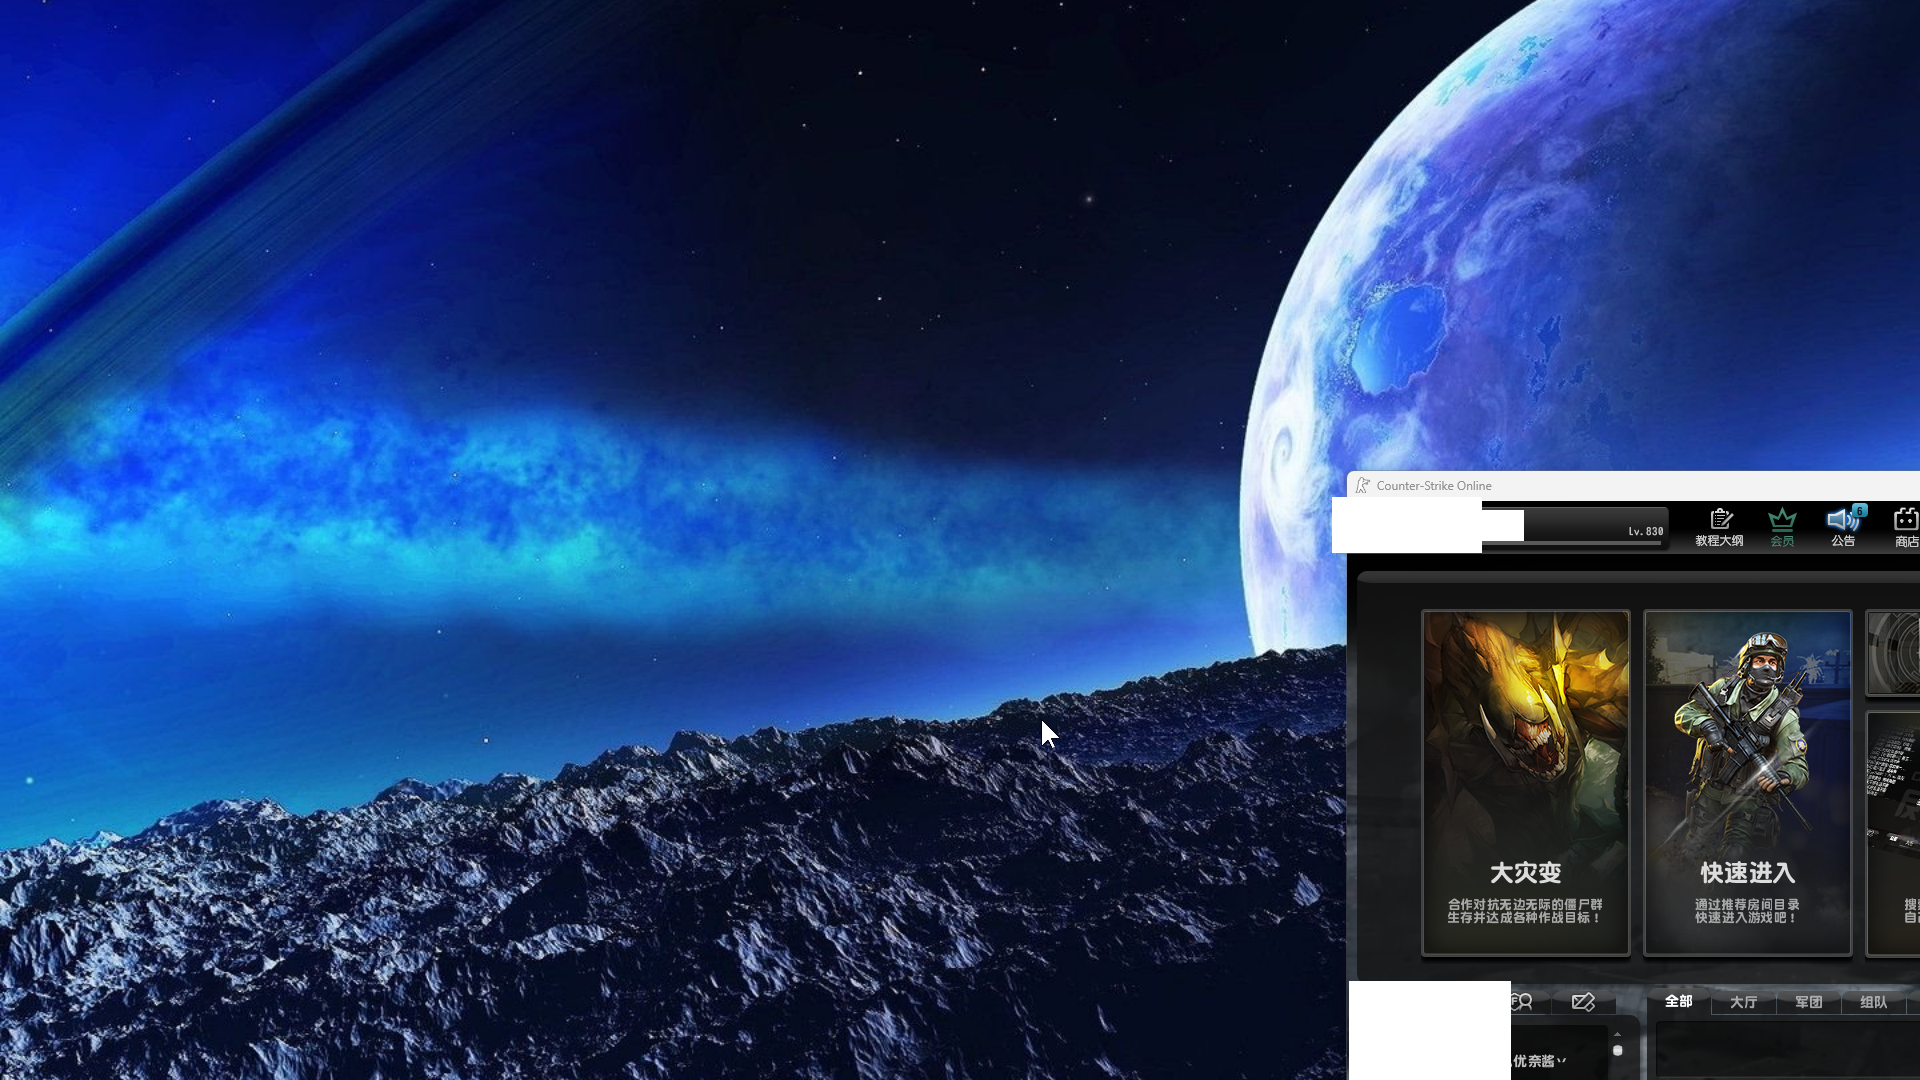
\includegraphics[width=\textwidth]{documents/assets/before-make-borderless.png}
    \caption{无边框窗口化前(窗口可随意移动)}
    \label{ch2fig-before-make-borderless}
\end{figure}

\begin{figure}
    \Centering
    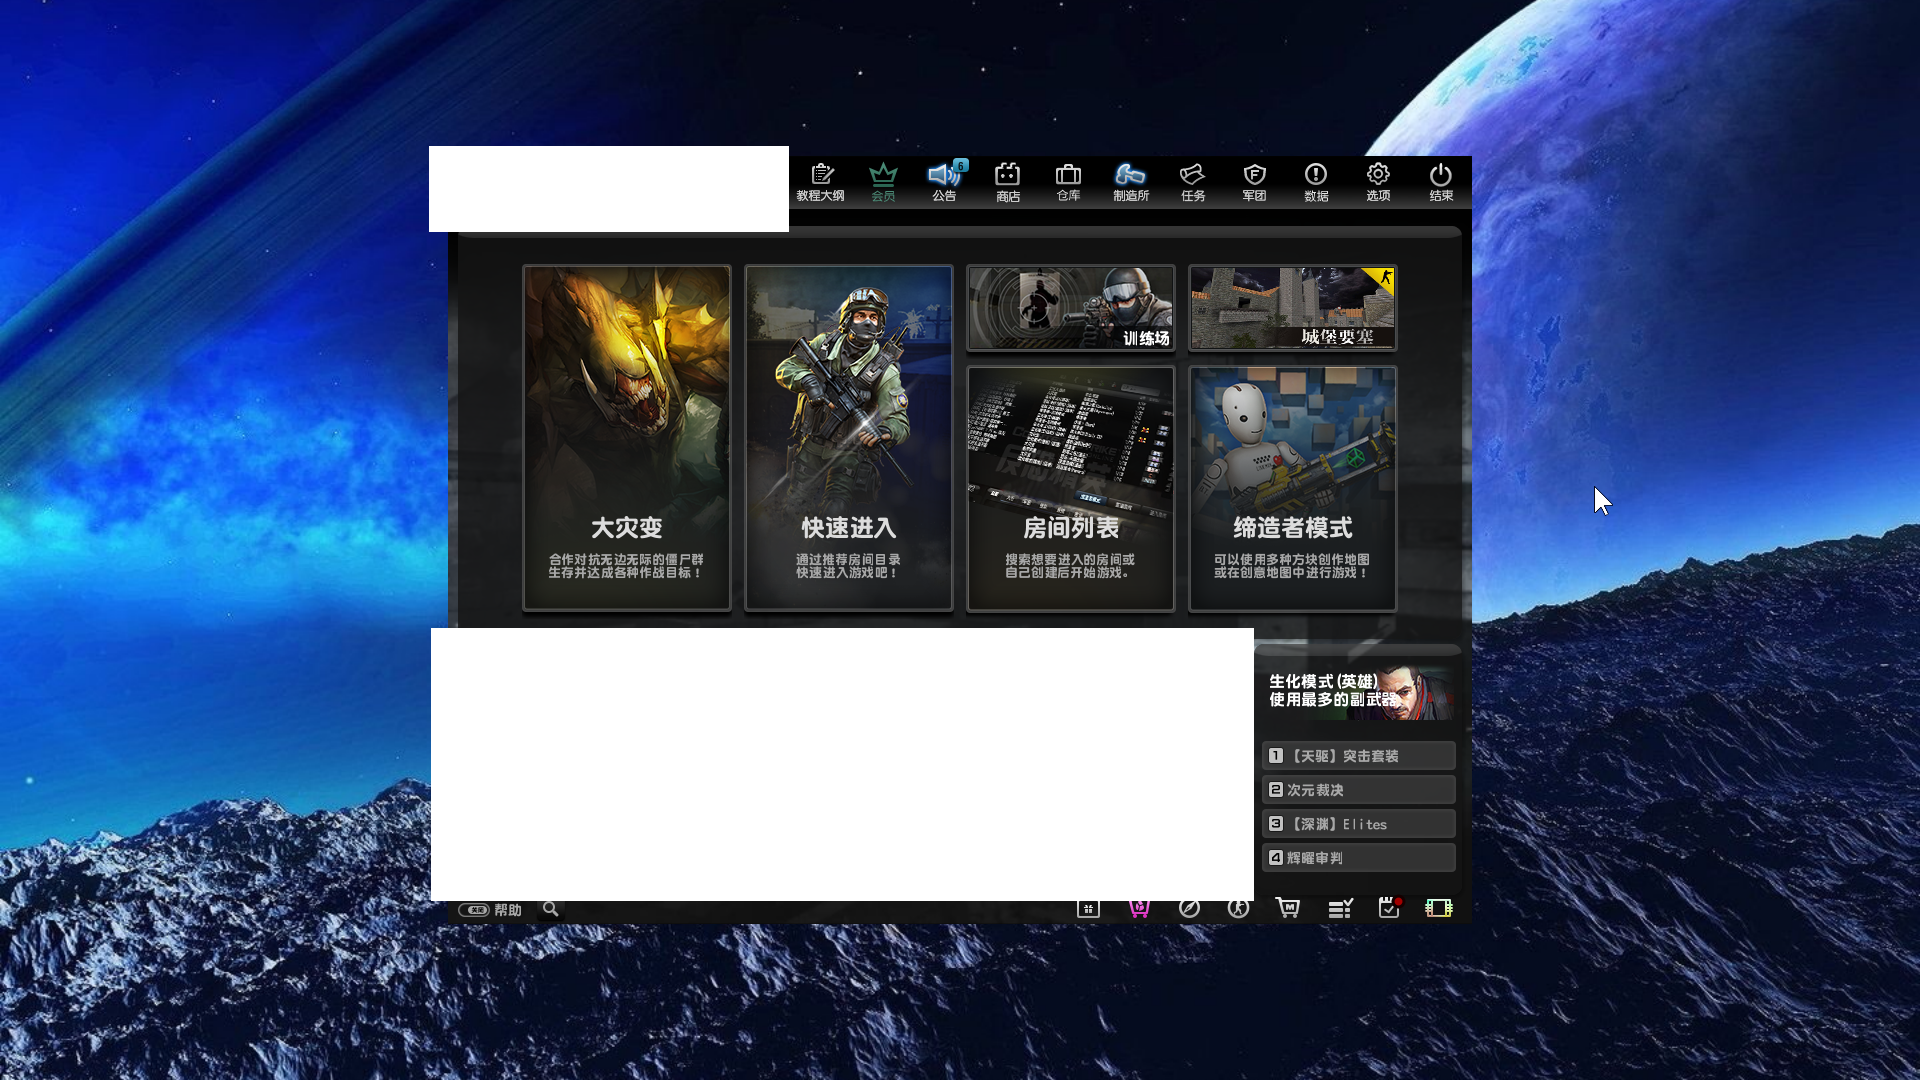
\includegraphics[width=\textwidth]{documents/assets/after-make-borderless.png}
    \caption{无边框窗口化后(窗口居中、标题栏去除、不可随意移动)}
    \label{ch2fig-after-make-borderless}
\end{figure}

有关 GamingTool 更多使用方法,参考 \href{https://gitee.com/silver1867/gaming-tool}{GamingTool 项目链接}。

在使用配置面板时,需要注意️\emotion{⏺️}代表录制按键按钮,按键录制完成后,需点击\emotion{⏹️}结束录制(图 \ref{ch2fig-about-recording})。

\begin{figure}[H]
    \Centering
    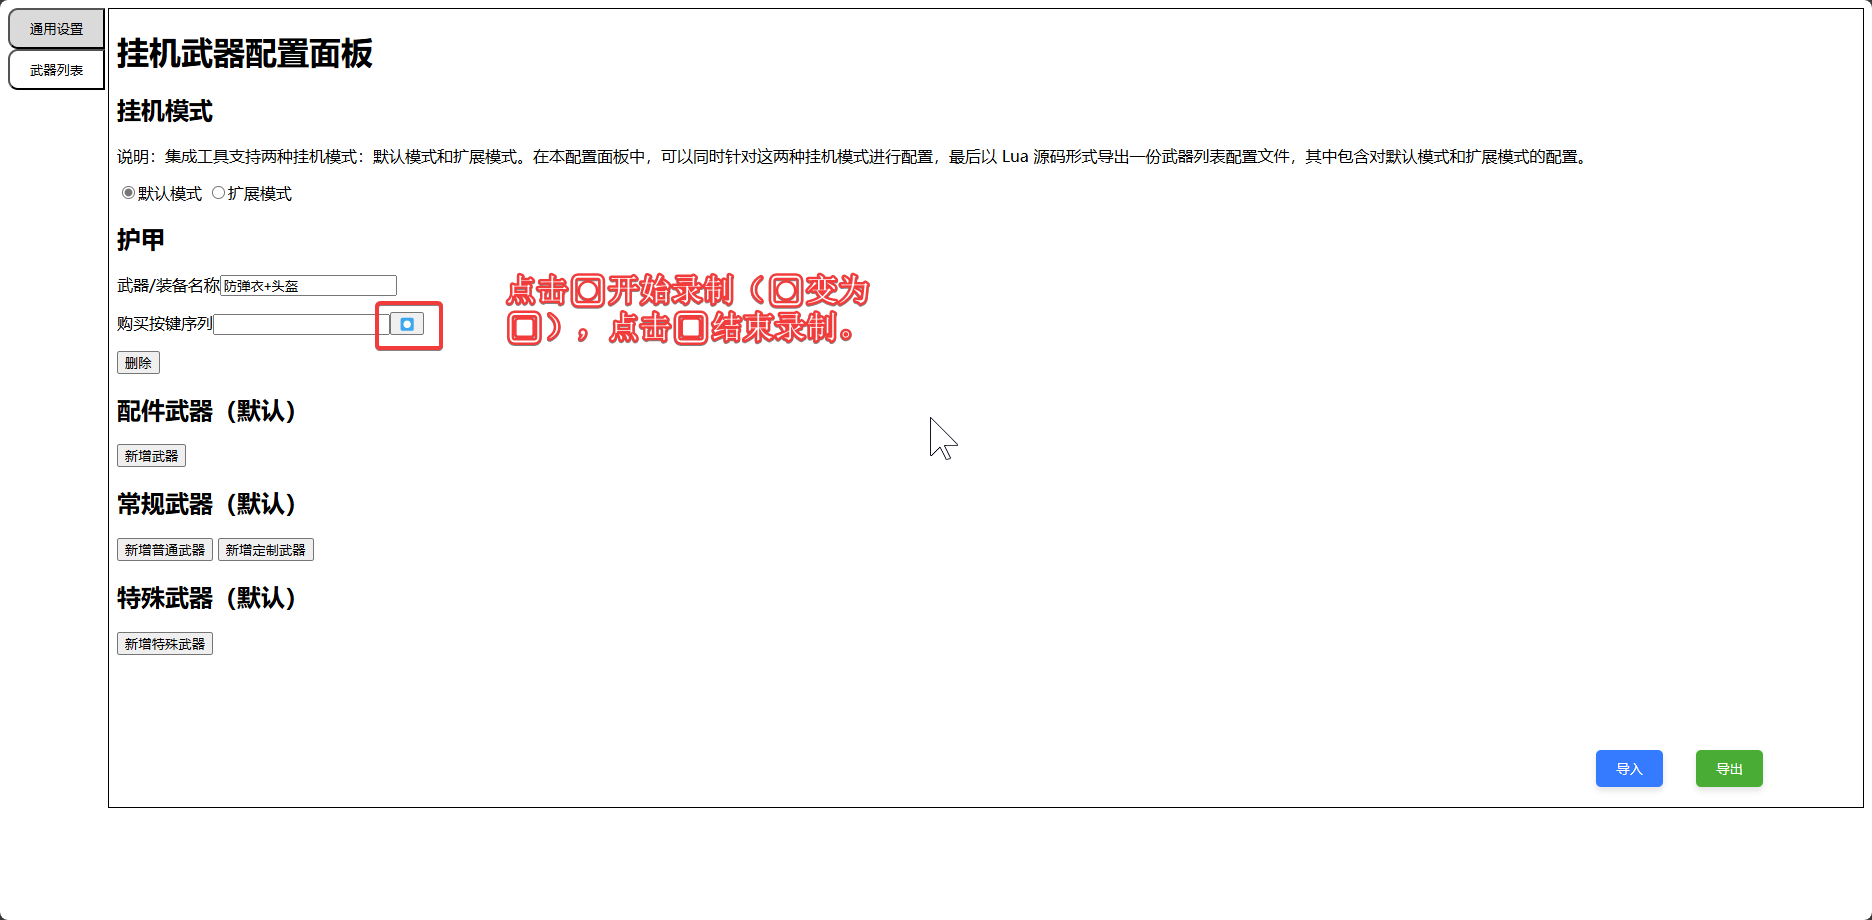
\includegraphics[width=\textwidth]{documents/assets/about_recording}
    \caption{导出配置文件}
    \label{ch2fig-about-recording}
\end{figure}

\subsection{通用设置}

将控制器调到模式 5 进行坐标定位。

v1.5 相较 v1.4 的其中一个重要改进在于重写了配置面板,点击访问\href{https://macrohard.fun/CSOL-Utilities/ConfigPanel}{CSOL 集成工具配置面板}进行配置:

所有的坐标均通过 5 模式坐标定位功能确定。
按照配置面板上的指引配置完成后,点击“导出”按钮生成配置文件,并将配置文件保存到 \lstinline{Executor} 目录下,保存时\textbf{\color{red}替换}原有的 \lstinline{Setting.lua} 文件。

\begin{figure}[H]
    \Centering
    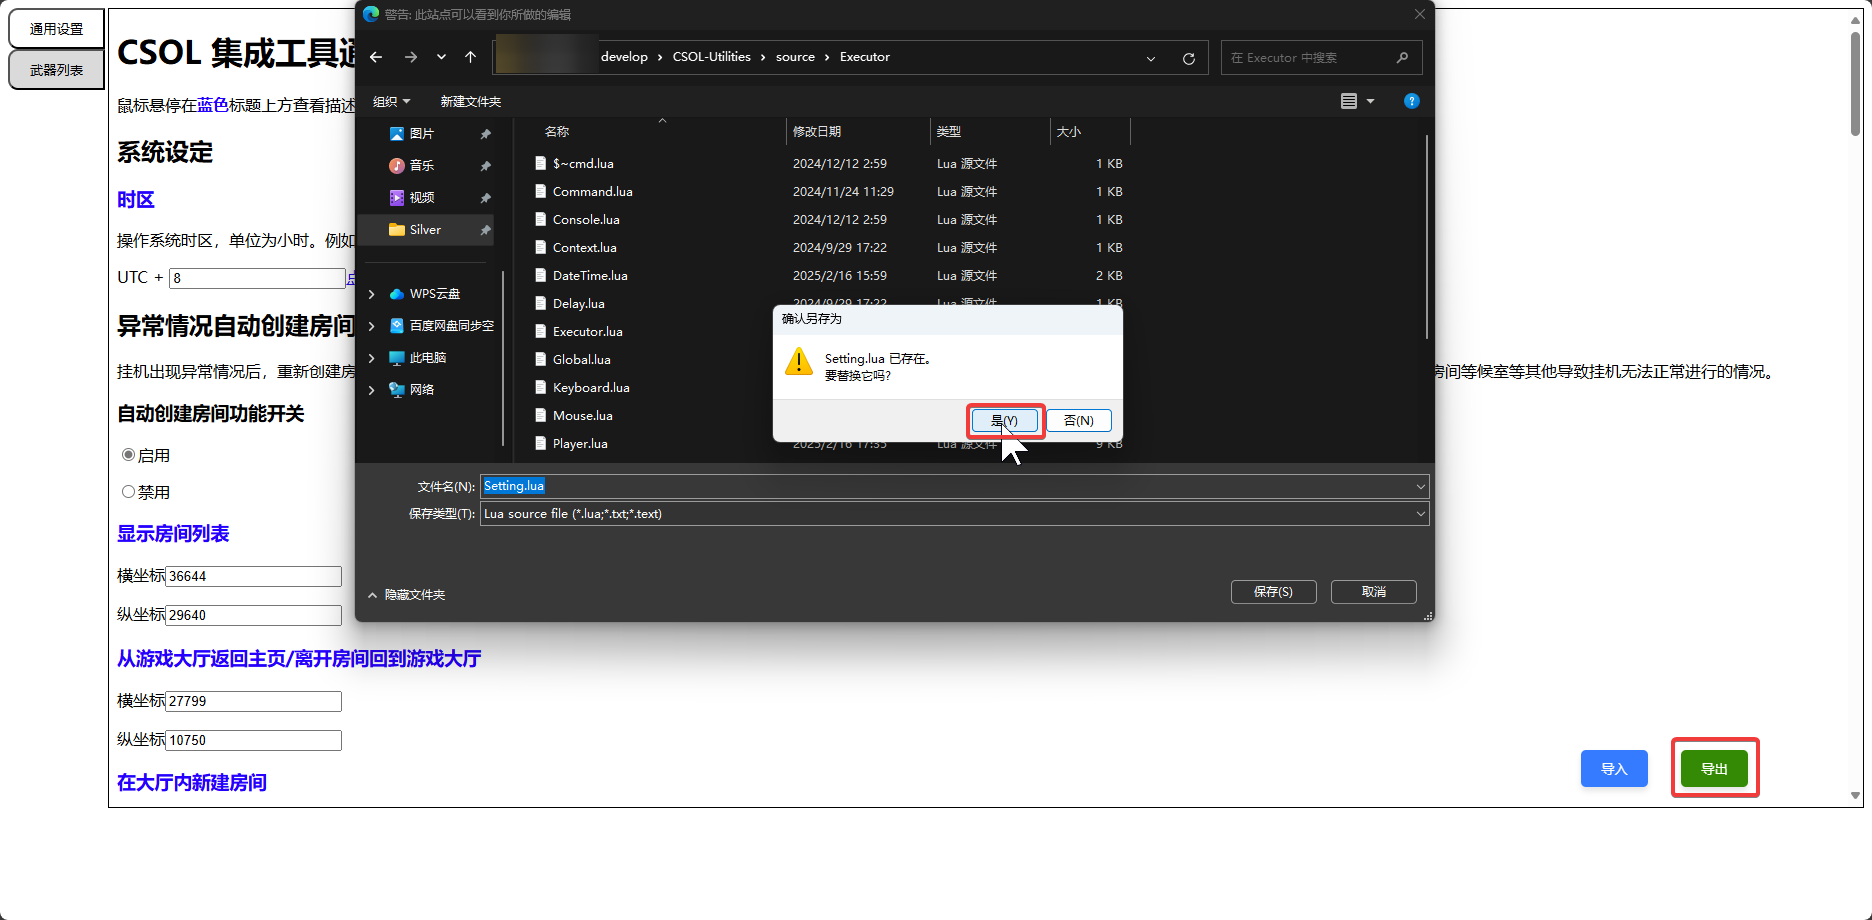
\includegraphics[width=\textwidth]{documents/assets/export_setting}
    \caption{导出配置文件}
    \label{ch2fig-export-setting}
\end{figure}

在通用设置面板中的“导入”按钮支持导入 \lstinline{Setting.lua} 文件。v1.5 版本配置面板对 v1.4 版本保持向下兼容,因此你可以向面板中导入 v1.4 版本的 \lstinline{Setting.lua},面板会自动将其转换为 v1.5 的配置。

若有未填写的必填字段,执行导出操作时会失败(配置面板出现相应提示)。

\begin{figure}[H]
    \Centering
    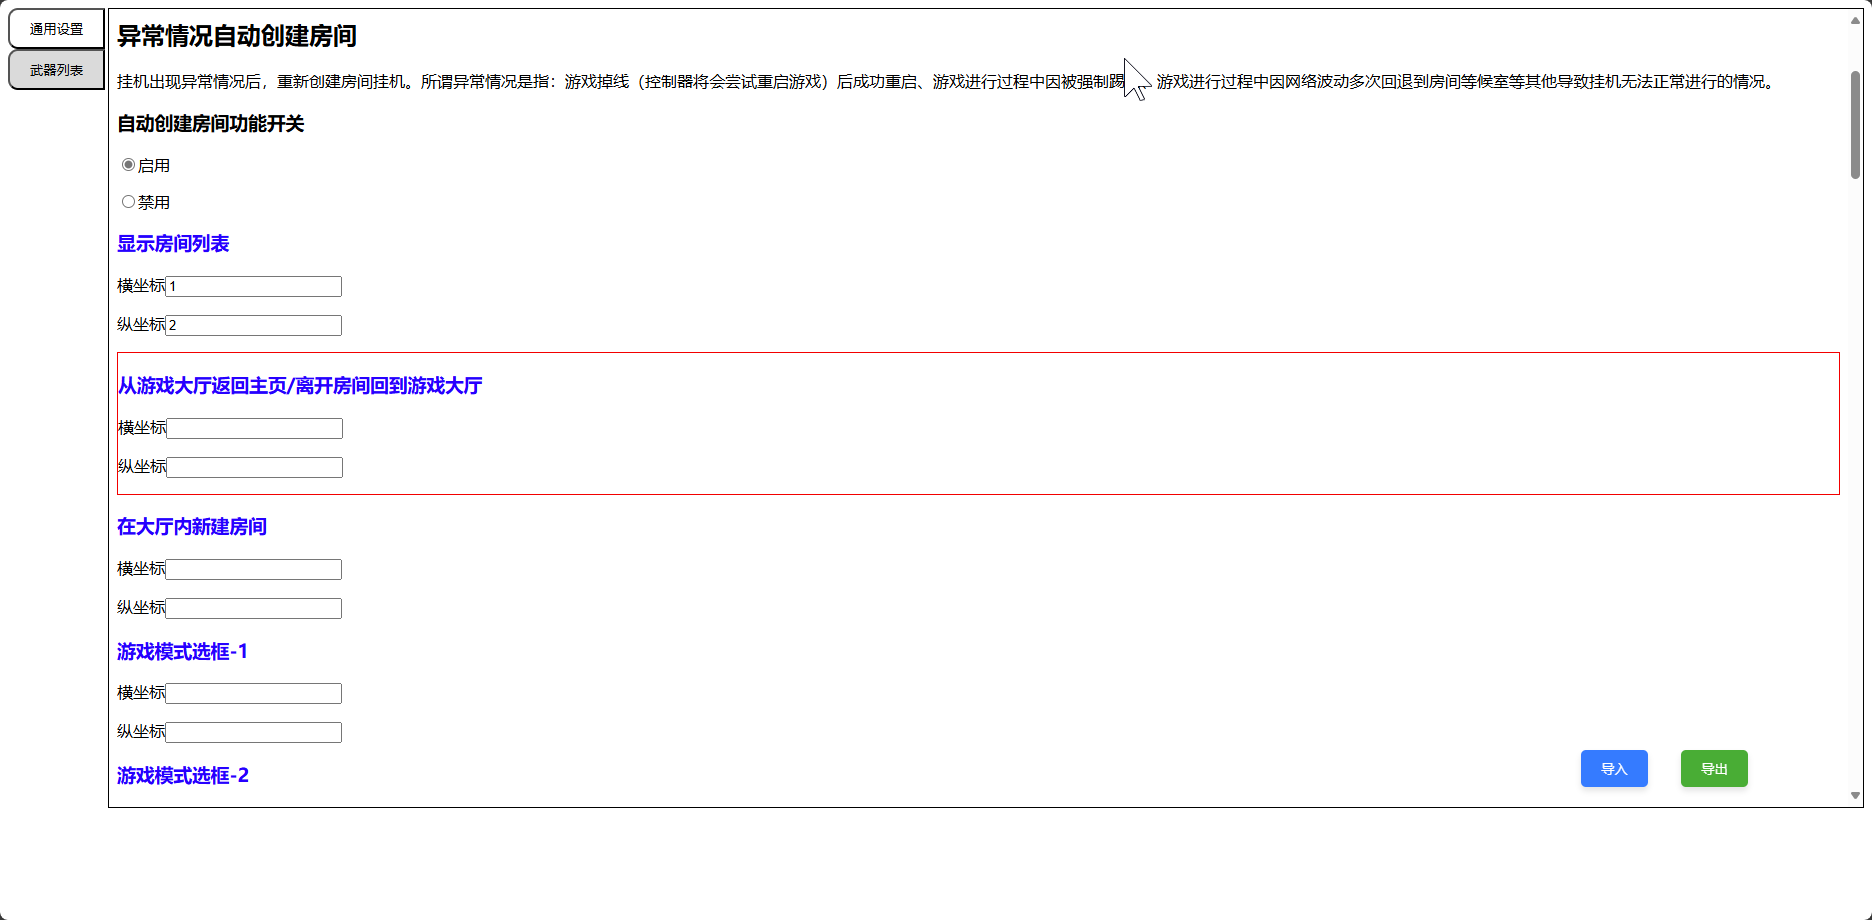
\includegraphics[width=\textwidth]{documents/assets/export_error}
    \caption{导出失败提示}
\end{figure}

\textbf{\color{red}注意:配置文件修改后后,需要在罗技软件中重新导入并运行以使配置生效。}

\subsection{挂机模式选择}

集成工具提供两种挂机模式,从 v1.5 起,两种挂机模式在功能上没有任何区别。二者唯一的区别在于:一号挂机模式为默认挂机模式,二号挂机模式为扩展挂机模式,\textbf{当使用扩展挂机模式进行挂机时,会先使用默认挂机模式进行一段时间的挂机操作(默认为 1 分钟),随后才切换至扩展挂机模式。}并且,在掉线重连后,挂机模式会被重置为默认挂机模式。\footnote{在未来的版本中,会新增控制器配置选项,届时可以对此进行配置。}

因此,默认挂机模式应该设置得较为保守,扩展挂机模式则建议设置丰富的武器列表。

在武器配置面板中,配件武器是指挂机过程中携带的辅助武器(如伤害生命配件的武器),需要注意:配件武器永远不会被使用。您可以指定任意数量的配件武器,但从实际情况出发,不建议指定超过三个。例如,只使用刀挂机,就指定三件配件武器。

常规武器是指采用常规方式进行攻击的武器,在配置面板中提供了“新增普通武器”和“新增定制武器”两种选项。\textbf{\color{red}所谓“普通”,是指使用左键或右键进行攻击。“定制”则是针对某些同时具备常规和非常规攻击方式的武器(如:万钧神威),对此类武器,配置面板提供了专门定制的武器使用逻辑,您只需要配置武器购买按键序列即可(在下拉框中选择武器时会自动填充武器名称)。}您可以指定\textbf{\color{red}任意数量}的常规武器,并且可以重复添加同一件武器,\textbf{在挂机过程中,挂机执行器会等概率地从中抽取一件使用一段时间,然后再抽取下一件武器,所以,某一件武器重复次数越多,被抽到的概率越大。}

\begin{figure}[H]
    \Centering
    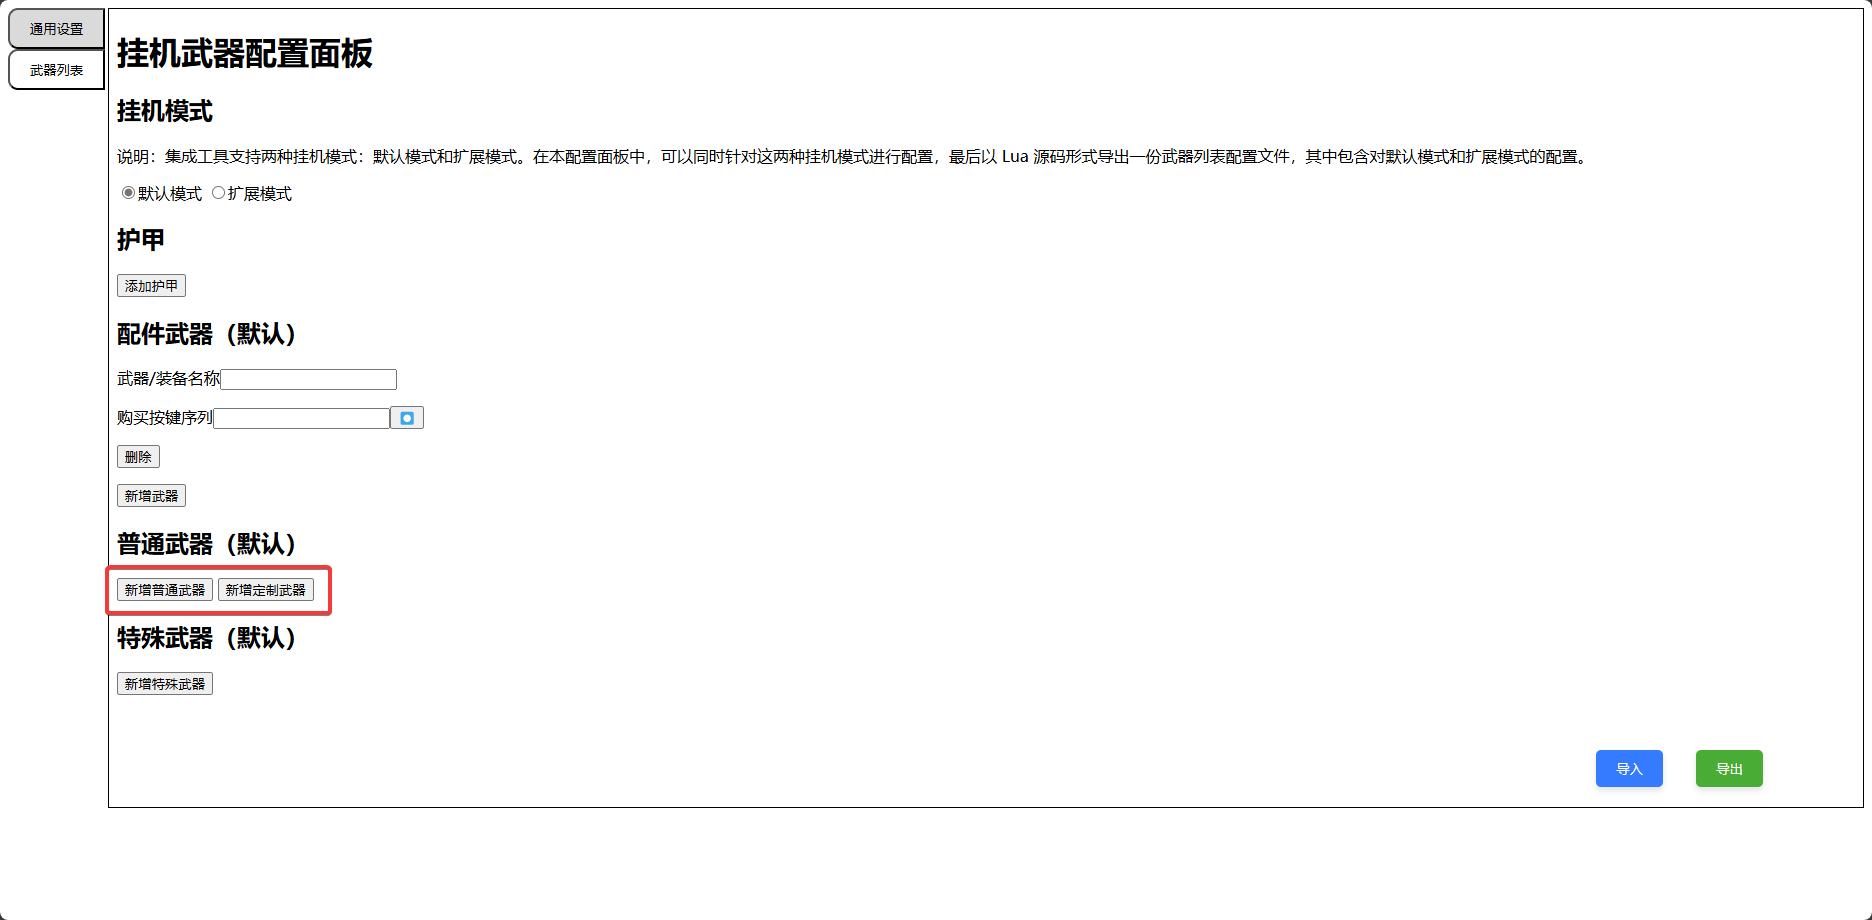
\includegraphics[width=\textwidth]{documents/assets/about_conventional_weapons}
    \caption{“添加普通武器”和“添加定制武器”}
\end{figure}

特殊武器是指像圣翼皓印这样采用特殊攻击方式的武器,其攻击方式与常规武器有本质不同,因此只提供定制化的配置。选择相应武器模板,并指定购买按键序列即可在挂机过程中使用特殊武器。

设置完成后,点击“导出”,保存 \lstinline{WeaponList.lua} 到 \lstinline{Executor} 目录下,覆盖原有的 \lstinline{WeaponList.lua} 文件。

对于 v1.4 版本的用户,需注意 v1.5 版本的配置面板向下兼容 v1.4 版本的武器列表配置文件,但对于定制武器不会自动套用最新的武器模板,因此导入后若需要使用最新的武器模板则需要手动指定。

\begin{figure}[H]
    \Centering
    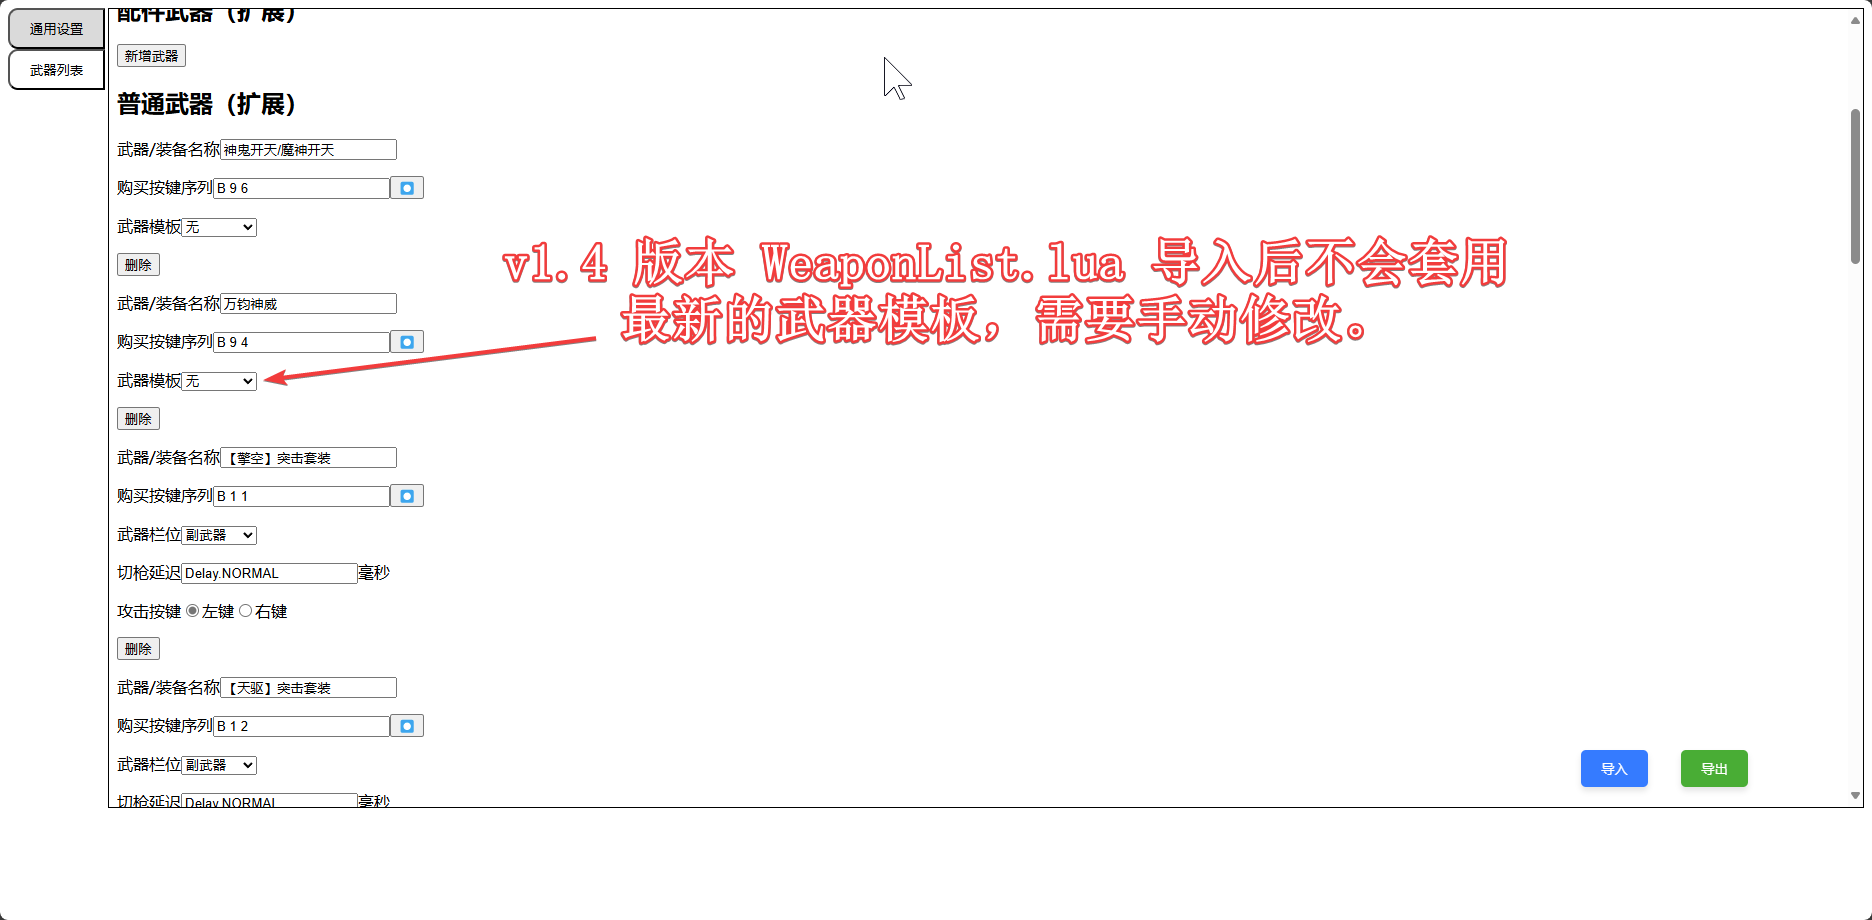
\includegraphics[width=\textwidth]{documents/assets/weapons_for_previous_versions}
    \caption{“添加普通武器”和“添加定制武器”}
\end{figure}

对于具有一定编程经验的用户,阅读完本节内容后可以参阅\nameref{section_advanced_usage}了解更多自定义使用方法。\footnote{此部分尚需完善。}

\subsection{使用方法}

上述配置无误后,进入一个挂机房间,按 \lstinline{Ctrl} \lstinline{Alt} \lstinline{Shift} \lstinline{1} 或 \lstinline{Ctrl} \lstinline{Alt} \lstinline{Shift} \lstinline{2} 选择 1 模式或 2 模式开始挂机。